\documentclass[11pt,a4paper,dvipdfmx]{jsarticle}

%定数
\newcommand{\accessToken}{アクセストークン \index{あくせすとーくん@アクセストークン}}
\newcommand{\bj}{「BaconJam」\index{baconjam@BaconJam}}
\newcommand{\bracketref}[1]{(\ref{#1}) {\footnotesize (P.\pageref{#1})}}
\newcommand{\change}{\colorbox{orange}{\textcolor{white}{\textbf{変更}}}\xdotfill{1pt}[orange]}
\newcommand{\currentVersion}{\texttt{Ver1.2.3}}
\newcommand{\fix}{\colorbox{red}{\textcolor{white}{\textbf{修正}}}\xdotfill{1pt}[red]}
\newcommand{\imageref}[1]{図\ref{#1}}
\newcommand{\mi}{\texttt{Misskey} \index{misskey@Misskey}}
\newcommand{\new}{\colorbox{teal}{\textcolor{white}{\textbf{新規}}}\xdotfill{1pt}[teal]}
\newcommand{\nowplaying}{「なうぷれ投稿」 \index{なうぷれとうこう@なうぷれ投稿}}
\newcommand{\spotifydashboard}{\href{https://developer.spotify.com/dashboard}{Dashboard}}
\newcommand{\ttbox}[1]{\ovalbox{\texttt{#1}}}
\newcommand{\ver}[1]{\texttt{Ver#1}}
\newcommand{\clientId}{\texttt{ClientID} \index{clientid@ClientID}}
\newcommand{\clientSecret}{\texttt{ClientSecret} \index{clientsecret@ClientSecret}}

%目次に節まで表示
\setcounter{tocdepth}{3}

\usepackage{amssymb}
\usepackage{okumacro}
\usepackage{amsmath,amssymb}
\usepackage{bm}
\usepackage[dvipdfm]{graphicx}
\usepackage[dvipdfm]{color}
\usepackage{ascmac}
\usepackage[dvipdfmx]{hyperref}
\usepackage{pdfpages}
\usepackage{pxjahyper}
\usepackage{makeidx}
\usepackage{fancybox}
\usepackage{caption}
\usepackage{xhfill}

\hypersetup{% hyperrefオプションリスト
setpagesize=false,
 bookmarksnumbered=true,%
 bookmarksopen=true,%
 colorlinks=true,%
 linkcolor=blue,
 citecolor=red,
}

\makeindex

\title{\bj (\currentVersion) 操作説明書 }
\author{くろいぬ/Falhong-Cha}
\date{最終更新日:\today}

\begin{document}
\renewcommand{\labelenumi}{(\arabic{enumi})}

\begin{titlepage}
	\maketitle\thispagestyle{empty}
\end{titlepage}
\tableofcontents

\clearpage
\section{Spotifyとの連携 \index{spotify@Spotify}}
\label{sec:spotify1}
    \subsection{Spotify側の設定}
    \label{sec:spotify2}
        \subsubsection{Spotify for Developersの認証 \index{spotifyfordevelopers@Spotify for Developers}}
        \label{sec:spotify3}
            \begin{enumerate}
                \item \href{https://developer.spotify.com}{Spotify for Developers}にアクセスし、ご利用のSpotifyアカウントでログインしてください。
                \label{item:spotify1}
                \item アカウント名を押下してメニューを表示し、\ttbox{Dashboard}を押下して\spotifydashboard へ移動してください。
                \label{item:spotify2}
                    \begin{figure}[htbp]
                        \centering
                        \fbox{
                            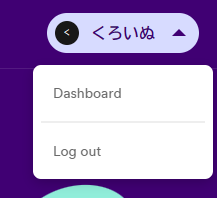
\includegraphics[width=5cm]{./pictures/spotify1.png}
                        }
                        \caption{メニューのDashboard}
                        \label{img:spotify1}
                    \end{figure}

                \item \spotifydashboard で
                    \begin{screen}
                        \texttt{You need to verify your email address (アカウントに登録されているメールアドレス) before you can create an app.}
                    \end{screen}
                    と表示されている部分の\ttbox{Update email address}を押下してください。
                \label{item:spotify3}
                    \begin{figure}[htbp]
                        \centering
                        \fbox{
                            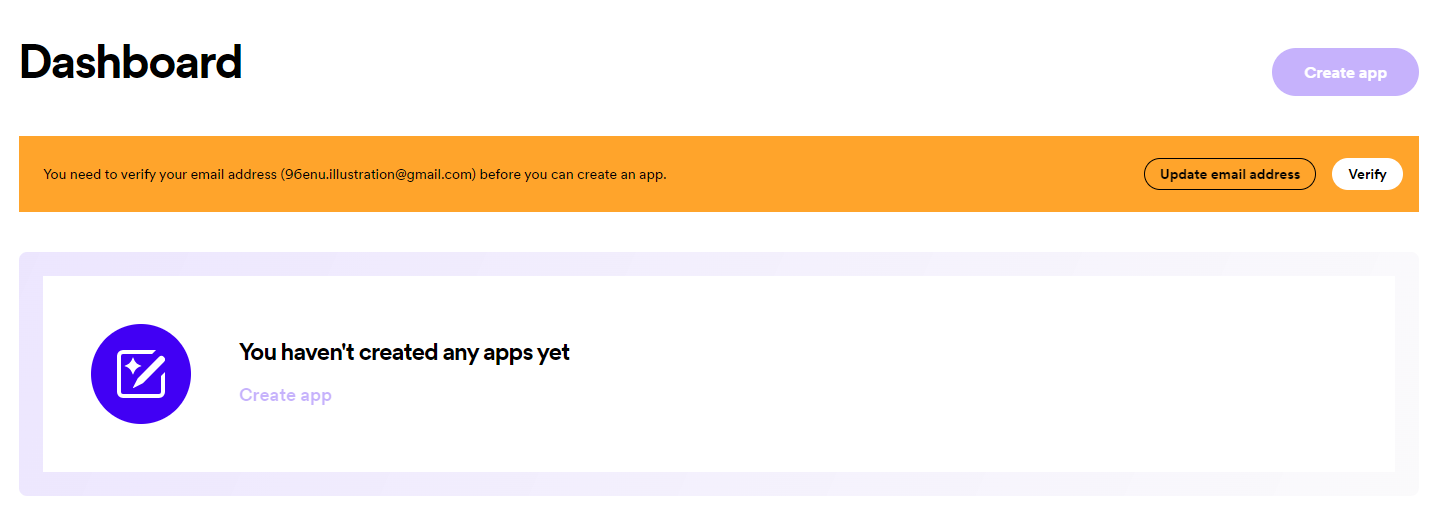
\includegraphics[width=\linewidth]{./pictures/spotify2.png}
                        }
                        \caption{DashboardのUpdate email address}
                        \label{img:spotify2}
                    \end{figure}

                \newpage
                \item \bracketref{item:spotify3}の実行後、アカウントに登録されているメールアドレスに\texttt{no-reply@spotify.com}から\imageref{img:spotify3}のようなセキュリティ確認のメールが送られてくるので、\ttbox{メールアドレスを確認する}を押下してください。
                \label{item:spotify4}
                    \begin{figure}[htbp]
                        \centering
                        \fbox{
                            \includegraphics[width=6cm]{./pictures/Spotify3.png}
                        }
                        \caption{セキュリティ確認のメール}
                        \label{img:spotify3}
                    \end{figure}

                \newpage
                \item ブラウザ上で\imageref{img:spotify4}のようなページが表示されたら、\spotifydashboard に戻ってください。
                \label{item:spotify5}
                    \begin{figure}[htbp]
                        \centering
                        \fbox{
                            \includegraphics[width=6cm]{./pictures/Spotify4.png}
                        }
                            \caption{認証完了画面}
                        \label{img:spotify4}
                    \end{figure}
                \item \spotifydashboard で、\bracketref{item:spotify3}時点では押下できなかった\ttbox{Create app}が押下できるようになっていれば、認証完了です。
            \end{enumerate}

        \newpage
        \subsubsection{Spotifyと\bj 接続用appの作成}
        \label{sec:spotify4}
            \begin{enumerate}
                \item \spotifydashboard の\ttbox{Create app}を押下してください。
                \label{item:spotify6}
                    \begin{figure}[htbp]
                        \centering
                        \fbox{
                            \includegraphics[width=\linewidth]{./pictures/Spotify5.png}
                        }
                        \caption{\spotifydashboard のCreate app}
                        \label{img:spotify5}
                    \end{figure}

                \newpage
                \item \imageref{img:spotify6}のようなapp作成ページが表示されるので、以下を参考に値を設定してください。
                \label{item:spotify7}
                    \begin{figure}[htbp]
                        \centering
                        \fbox{
                            \includegraphics[width=\linewidth]{./pictures/Spotify6.png}
                        }
                        \caption{app作成ページ}
                        \label{img:spotify6}
                    \end{figure}
                    \begin{itemize}
                        \item[\texttt{App name}] なんらかの値を設定してください\footnote{自由な値で構いませんが、\bj 用のappであることが分かるような名前の設定を推奨します。}。
                        \item[\texttt{App description}] なんらかの値を設定してください。
                        \item[\texttt{Website}] 空欄で構いません。
                        \item[\texttt{Redirect URIs}] 必ず\texttt{http://localhost}という値を設定してください。
                        \item[\texttt{Bundle IDs}] 空欄で構いません。
                        \item[\texttt{Android packages}] 空欄で構いません。
                        \item[\texttt{APIs used}] 以下にチェックを入れてください。
                            \begin{itemize}
                                \item \texttt{Android}
                                \item \texttt{Web API}
                            \end{itemize}
                    \end{itemize}

                \newpage
                \item \bracketref{item:spotify7}の項目設定が完了したら、
                \label{item:spotify8}
                    \begin{screen}
                        \texttt{I understand and agree with Spotify's Developer Terms of Service and Design Guidelines}
                    \end{screen}
                    にチェックを入れ、\ttbox{save}を押下してください。

                \item \imageref{img:spotify7}のようなapp Homeページが表示されたら、作成完了です。
                \label{item:spotify9}
                    \begin{figure}[htbp]
                        \centering
                        \fbox{
                            \includegraphics[width=\linewidth]{./pictures/Spotify7.png}
                        }
                        \caption{app Homeページ}
                        \label{img:spotify7}
                    \end{figure}
            \end{enumerate}

        \newpage
        \subsubsection{接続に必要な情報の取得}
        \label{sec:spotify5}
            \begin{enumerate}
                \item \ref{sec:spotify4}で作成したappのHomeページにアクセスし、\ttbox{Settings}を押下してBasic Informationページに移動してください。
                \label{item:spotify10}

                \item ページ上部の\texttt{Client ID}が表示されている枠の\texttt{View client secret}を押下して、\texttt{Client secret}を表示してください。
                \label{item:spotify11}
                    \begin{figure}[htbp]
                        \centering
                        \fbox{
                            \includegraphics[width=\linewidth]{./pictures/Spotify8.png}
                        }
                        \caption{Basic Informationページ上部(Client secretを表示する前)}
                        \label{img:spotify8}
                    \end{figure}
                    \begin{figure}[htbp]
                        \centering
                        \fbox{
                            \includegraphics[width=\linewidth]{./pictures/Spotify9.png}
                        }
                        \caption{Basic Informationページ上部(Client secretを表示した後)}
                        \label{img:spotify9}
                    \end{figure}

                \item 以下の項目を控えてください。
                \label{item:spotify12}
                    \begin{itemize}
                        \item \texttt{Client ID}
                        \item \texttt{Client secret}
                    \end{itemize}
            \end{enumerate}

            \begin{itembox}[c]{\ttbox{!注意!}}
                \texttt{Client ID},\texttt{Client secret}は他人に知られないように管理してください。アカウントへの不正アクセス・乗っ取り等が発生する危険があります。
            \end{itembox}

    \newpage
    \subsection{\bj 側の設定}
    \label{sec:spotify6}
        \begin{enumerate}
            \item 設定画面の\ttbox{Spotify接続設定(プレビュー版)}を押下して、設定項目を展開してください。
                \begin{figure}[htbp]
                    \begin{minipage}[b]{0.45\linewidth}
                        \centering
                        \fbox{
                            \includegraphics[width=5cm]{./pictures/Spotify10.png}
                        }
                        \caption{展開前}
                        \label{img:spotify10}
                    \end{minipage}
                    \begin{minipage}[b]{0.45\linewidth}
                        \centering
                        \fbox{
                            \includegraphics[width=5cm]{./pictures/Spotify11.png}
                        }
                        \caption{展開後}
                        \label{img:spotify11}
                    \end{minipage}
                    \caption*{Spotify接続設定(\currentVersion)}
                \end{figure}

            \newpage
            \item \ref{sec:spotify5} \bracketref{item:spotify12}で控えた\texttt{Client ID},\texttt{Client secret}を\ttbox{Spotify接続設定(プレビュー版)}に入力してください。
                \begin{figure}[htbp]
                    \centering
                    \fbox{
                        \includegraphics[width=5cm]{./pictures/Spotify12.png}
                    }
                    \caption{\texttt{Client ID},\texttt{Client secret}を入力}
                    \label{img:spotify12}
                \end{figure}

            \newpage
            \item \ttbox{Spotify接続設定(プレビュー版)}の\ttbox{接続テスト}ボタンが押下できるようになるので、押下して認証ページへアクセスしてください。
            \item \imageref{img:spotify13}のような認証ページが表示されるので、\ttbox{同意する}を押下してください。
                \begin{figure}[htbp]
                    \centering
                    \fbox{
                        \includegraphics[width=5cm]{./pictures/Spotify13.png}
                    }
                    \caption{認証ページ}
                    \label{img:spotify13}
                \end{figure}

            \newpage
            \item 認証ページが閉じ、\imageref{img:spotify14}のような成功ダイアログが表示されたらSpotify側の準備は完了です\footnote{ダイアログ内のユーザー名がご自身のアカウントと一致していることを確認してください}。
                \begin{figure}[htbp]
                    \centering
                    \fbox{
                        \includegraphics[width=5cm]{./pictures/Spotify14.png}
                    }
                    \caption{認証ページ}
                    \label{img:spotify14}
                \end{figure}
        \end{enumerate}

    \newpage
    \subsection{Spotify連携時の挙動について}
    \label{sec:spotify7}
    \begin{itemize}
        \item 約1分に一度、Spotifyで再生中の曲を確認し\mi への\nowplaying を行います。
        \item 以下のいずれかに該当する場合、\nowplaying を行いません。
        \begin{itemize}
            \item 再生中の曲がない
            \item \mi の\accessToken が設定されていない
            \item \nowplaying が有効になっていない
            \item 前回の\nowplaying と曲名・アーティスト名が変化していない
            \item スマートフォンがネットワークに接続されていない
            \item スマートフォンがロック状態になっている\footnote{ディスプレイを常時表示設定にすることで、解決する場合があります}
        \end{itemize}
    \end{itemize}


\newpage
\section{リリースノート}
\subsection*{バージョンコード2(1.0.0)}
\begin{itemize}
    \item[リリース日] 2024年3月28日
\end{itemize}

\new
\begin{itemize}
    \item クローズドテストを開始しました。
\end{itemize}

\change \par
\fix

\newpage
\subsection*{バージョンコード3(1.1.0)}
\addcontentsline{toc}{subsection}{バージョンコード3(1.1.0)}
\begin{itemize}
    \item[リリース日] 2024年4月7日
\end{itemize}

\new
\begin{itemize}
    \item \nowplaying の公開範囲を以下から選択できる機能を追加しました。
        \begin{enumerate}
            \item パブリック(全てのユーザーに公開)
            \item ホーム(ホームタイムラインのみに公開)
            \item フォロワー(自分のフォロワーのみに公開)
            \item チャンネル\footnote{チャンネルIDの設定が必要です}
        \end{enumerate}
    \item Spotifyとの連携機能(プレビュー版)を追加しました。
    \item 設定画面に\ttbox{設定をリセットする}ボタンを追加しました。
\end{itemize}

\change
\begin{itemize}
    \item \nowplaying の際に以下の順にアーティスト名を取得し、最初に見つかったものを表示するように変更しました。
        \begin{enumerate}
            \item アルバムアーティスト名
            \item トラックアーティスト名
            \item 著者名
            \item 作者名
        \end{enumerate}
    \item \mi のアクセストークンが空欄の場合、\ttbox{テスト接続}ボタンを押下できないように変更しました。
    \item 設定画面の各種項目を折りたためるようにUIを変更しました。
\end{itemize}

\fix
\begin{itemize}
    \item ランキング画面の不要な\ttbox{TEST}ボタンを削除しました。
    \item 初回インストール時に投稿パターンの初期値が設定されておらず、\nowplaying できない不具合を修正しました。
\end{itemize}

\newpage
\subsection*{バージョンコード4(1.1.1)}
\addcontentsline{toc}{subsection}{バージョンコード4(1.1.1)}
\begin{itemize}
    \item[リリース日] 2024年4月8日
\end{itemize}

\new \par
\change
\begin{itemize}
    \item \mi との連携方法を変更しました。
\end{itemize}

\fix
\begin{itemize}
    \item 投稿パターン選択用ドロップダウンの挙動の不具合を修正しました。
\end{itemize}

\newpage
\subsection*{バージョンコード5(1.1.2)}
\begin{itemize}
    \item[リリース日] 2024年4月8日
\end{itemize}

\new \par
\change \par
\fix
\begin{itemize}
    \item \mi との連携操作の不具合を修正しました。
\end{itemize}

\newpage
\subsection*{バージョンコード6(1.1.3)}
\begin{itemize}
    \item[リリース日] 2024年4月8日
\end{itemize}

\new \par
\change \par
\fix
\begin{itemize}
    \item \nowplaying 時の挙動不具合を修正しました。
\end{itemize}

\newpage
\subsection*{バージョンコード7(1.2.0)}
\begin{itemize}
    \item[リリース日] 2024年4月8日
\end{itemize}

\new \par
\change
\begin{itemize}
    \item \nowplaying の投稿先チャンネルを名称またはIDで検索して指定できるように変更しました。
    \item \bj 全体のフォントを\href{https://fonts.google.com/specimen/Murecho?subset=japanese}{Murecho}に変更しました。
\end{itemize}

\fix

\newpage
\subsection*{バージョンコード8(1.2.1)}
\addcontentsline{toc}{subsection}{バージョンコード8(1.2.1)}
\begin{itemize}
    \item[リリース日] 2024年4月11日
\end{itemize}

\new \par
\change \par
\fix
\begin{itemize}
    \item \clientId ,\clientSecret を入力した際の\ttbox{接続テスト}ボタンの挙動の不具合を修正しました。
\end{itemize}


\newpage
\subsection*{バージョンコード9(1.2.2)}
\addcontentsline{toc}{subsection}{バージョンコード9(1.2.2)}
\begin{itemize}
    \item[リリース日] 2024年4月12日
\end{itemize}

\new
\begin{itemize}
    \item Spotifyの曲を投稿する際、曲のURLを添付する機能を追加しました。
\end{itemize}

\change
\begin{itemize}
    \item \nowplaying のオンオフを変更した際、トーストメッセージを表示するように変更しました。
\end{itemize}

\fix
\begin{itemize}
    \item \nowplaying のオンオフがSpotifyの投稿機能と連動しない不具合を修正しました。
\end{itemize}


\newpage
\subsection*{バージョンコード10(1.2.3)}
\addcontentsline{toc}{subsection}{バージョンコード10(1.2.3)}
\begin{itemize}
    \item[リリース日] 2024年4月13日
\end{itemize}

\new \par
\change
\begin{itemize}
    \item ハンバーガーメニュー内の広告をテスト用から実際の広告に変更しました。
\end{itemize}

\fix


\newpage
\subsection*{バージョンコード11(1.2.4)}
\addcontentsline{toc}{subsection}{バージョンコード11(1.2.4)}
\begin{itemize}
    \item[リリース日] 2024年4月14日
\end{itemize}

\new \par
\change
\begin{itemize}
    \item ハンバーガーメニュー内のUIを変更しました。
\end{itemize}

\fix


\newpage
\subsection*{バージョンコード12(1.2.5)}
\addcontentsline{toc}{subsection}{バージョンコード12(1.2.5)}
\begin{itemize}
    \item[リリース日] 2024年4月15日
\end{itemize}

\new \par
\change \par
\fix
\begin{itemize}
    \item 起動できなくなる不具合を修正しました。
\end{itemize}



\newpage
\subsection*{バージョンコード13(1.2.6)}
\addcontentsline{toc}{subsection}{バージョンコード13(1.2.6)}
\begin{itemize}
    \item[リリース日] 2024年4月15日
\end{itemize}

\new \par
\change \par
\fix
\begin{itemize}
    \item 軽微な修正を行いました。
\end{itemize}



\newpage
\subsection*{バージョンコード16(1.2.9)}
\addcontentsline{toc}{subsection}{バージョンコード16(1.2.9)}
\begin{itemize}
    \item[リリース日] 2024年4月16日
\end{itemize}

\new
\begin{itemize}
    \item ハンバーガーメニューに連携している\mi のプロフィールを表示する機能を追加しました。
    \item ハンバーガーメニューに感想用Googleフォームへのリンクを追加しました。
\end{itemize}

\change \par
\fix
\begin{itemize}
    \item 軽微なUIの修正を行いました。
\end{itemize}



\newpage
\subsection*{バージョンコード21(1.3.4)}
\addcontentsline{toc}{subsection}{バージョンコード21(1.3.4)}
\begin{itemize}
    \item[リリース日] 2024年4月23日
\end{itemize}

\new
\begin{itemize}
    \item プレイリスト作成・再生機能を追加しました。
\end{itemize}

\change
\begin{itemize}
    \item クローズドテストから製品版(一般公開)にリリース先を変更しました。
\end{itemize}

\fix
\begin{itemize}
    \item 軽微なUIの修正を行いました。
\end{itemize}



\newpage
\subsection*{バージョンコード23(1.3.6)}
\addcontentsline{toc}{subsection}{バージョンコード23(1.3.6)}
\begin{itemize}
    \item[リリース日] 2024年4月24日
\end{itemize}

\new
\begin{itemize}
    \item 前の曲へボタン、次の曲へボタンを追加しました。
\end{itemize}

\change
\begin{itemize}
    \item プレイリストを再生ボタン、音楽ファイルを再生ボタンの配置を変更しました。
    \item プレイリスト未作成の場合の画面デザインを変更しました。
    \item ランキングデータなしの場合の画面デザインを変更しました。
\end{itemize}

\fix


\newpage
\subsection*{バージョンコード24(1.3.7)}
\addcontentsline{toc}{subsection}{バージョンコード24(1.3.7)}
\begin{itemize}
    \item[リリース日] 2024年4月27日
\end{itemize}

\new
\begin{itemize}
    \item 曲名、アーティスト名、アルバム名の\verb|#|を\verb|#|に置換しハッシュタグ化を防ぐ処理を追加しました。
\end{itemize}

\change
\begin{itemize}
    \item \mi 連携、Spotify連携の画面をアプリ内ブラウザ表示から外部ブラウザ表示に変更しました。
\end{itemize}

\fix



\newpage
\subsection*{バージョンコード25(1.3.8)}
\addcontentsline{toc}{subsection}{バージョンコード25(1.3.8)}
\begin{itemize}
    \item[リリース日] 2024年4月28日
\end{itemize}

\new
\begin{itemize}
    \item \href{https://misskey-hub.net/ja/servers/}{Misskey Hubのサーバー一覧}に掲載されていないサーバーでも接続先として指定できる機能を追加しました。
    \item ライトテーマ・ダークテーマ変更時にポップアップ通知を表示する機能を追加しました。
\end{itemize}

\change
\begin{itemize}
    \item 接続先サーバー変更時に、カスタム絵文字を自動的に取得するように変更しました。
\end{itemize}

\fix



\newpage
\subsection*{バージョンコード26(1.3.9)}
\addcontentsline{toc}{subsection}{バージョンコード26(1.3.9)}
\begin{itemize}
    \item[リリース日] 2024年4月30日
\end{itemize}

\new
\begin{itemize}
    \item ハンバーガーメニューのアイコンを押下すると\mi のプロフィールにジャンプする機能を追加しました。
    \item \nowplaying の際に以下に含まれる\verb|:|を\verb|:|に置換し、カスタム絵文字の表示が崩れないようにする機能を追加しました。
        \begin{itemize}
            \item 曲名
            \item アーティスト名
            \item アルバム名
        \end{itemize}
\end{itemize}

\change

\fix



\newpage
\subsection*{バージョンコード27(1.4.0)}
\addcontentsline{toc}{subsection}{バージョンコード27(1.4.0)}
\begin{itemize}
    \item[リリース日] 2024年5月1日
\end{itemize}

\new

\change
\begin{itemize}
    \item サポート対象のandroid OSを13以上から5以上に拡張しました。
\end{itemize}

\fix



\newpage
\subsection*{バージョンコード28(1.4.1)}
\addcontentsline{toc}{subsection}{バージョンコード28(1.4.1)}
\begin{itemize}
    \item[リリース日] 2024年5月3日
\end{itemize}

\new
\begin{itemize}
    \item 外部ストレージの音楽ファイル読み込み機能を追加しました。
\end{itemize}

\change

\fix



\newpage
\section{各種連絡先}
\label{contact}
    \begin{itemize}
        \item[Misskey.io] \href{https://misskey.io/@96ENU}{\texttt{@96ENU}}
        \item[Twitter] \href{https://twitter.com/96ENU}{\texttt{@96ENU}}
        \item[Mail] \verb|96enu.illustration@gmail.com|
        \item[Discord]
            \begin{itemize}
                \item 個人:\verb|96ENU|
                \item \bj 用サーバ:\href{https://discord.gg/C3veaKqp}{Join to Server}
            \end{itemize}
    \end{itemize}

\newpage
\printindex
\end{document}